% Conceptual figure C1 -- WireGuard receive-path overview.
% Owner: narrative writer. Vector standalone TikZ; compiled to c1_recv_overview.pdf
% and included by paper/03-background-motivations.tex.
% Color semantics (Okabe-Ito, color-blind safe), reinforced by text labels and
% line styles: amber = pending/encrypted, teal = decrypted/ready,
% blue = the NAPI context, dark = ordering barrier.
\documentclass[border=3pt]{standalone}
\usepackage{tikz}
\usepackage[T1]{fontenc}
\usetikzlibrary{arrows.meta,positioning,fit,backgrounds}

\definecolor{cAmber}{HTML}{E69F00}
\definecolor{cTeal}{HTML}{009E73}
\definecolor{cBlue}{HTML}{0072B2}
\definecolor{cInk}{HTML}{222222}

\begin{document}
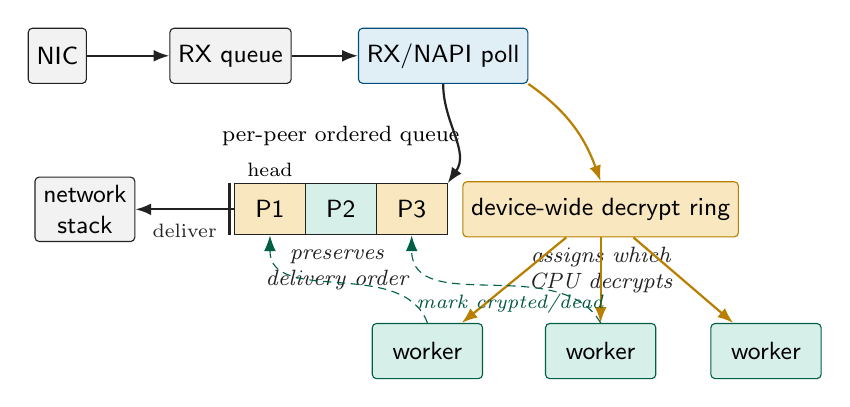
\begin{tikzpicture}[
  font=\sffamily\small,
  >={Latex[length=2mm]},
  box/.style={draw=cInk,rounded corners=1.5pt,minimum height=7mm,inner sep=3pt,align=center},
  hw/.style={box,fill=black!5},
  napi/.style={box,fill=cBlue!12,draw=cBlue!70!black},
  ring/.style={box,fill=cAmber!25,draw=cAmber!80!black,minimum width=26mm},
  worker/.style={box,fill=cTeal!16,draw=cTeal!60!black,minimum width=14mm},
  slot/.style={draw=cInk,minimum width=9mm,minimum height=6.5mm,inner sep=1pt},
  flow/.style={->,thick,cInk},
  assign/.style={->,thick,cAmber!80!black},
  setst/.style={->,densely dashed,cTeal!60!black},
  role/.style={font=\footnotesize\itshape,text=cInk}
]

% ---------- ingress row (y = 0) ----------
\node[hw]   (nic)  at (0,0)   {NIC};
\node[hw]   (rxq)  at (2.2,0) {RX queue};
\node[napi] (poll) at (4.9,0) {RX/NAPI poll};
\draw[flow] (nic) -- (rxq);
\draw[flow] (rxq) -- (poll);

% ---------- ordering path (y = -1.95): per-peer ordered queue ----------
\node[slot,fill=cAmber!25] (s1) at (2.7,-1.95) {P1};
\node[slot,fill=cTeal!16]  (s2) at (3.6,-1.95) {P2};
\node[slot,fill=cAmber!25] (s3) at (4.5,-1.95) {P3};
\node[font=\footnotesize] at (3.6,-1.02) {per-peer ordered queue};
\node[role,align=center] at (3.55,-2.72) {preserves\\delivery order};
\node[font=\scriptsize] at (2.7,-1.45) {head};
\draw[cInk,line width=1pt] ([xshift=-1.5pt]s1.north west) -- ([xshift=-1.5pt]s1.south west);

% ---------- assignment path: ring (right) + workers (bottom) ----------
\node[ring]   (ring) at (6.9,-1.95) {device-wide decrypt ring};
\node[role,align=center]   at (6.9,-2.72) {assigns which\\CPU decrypts};
\node[worker] (w0) at (4.7,-3.75) {worker};
\node[worker] (w1) at (6.9,-3.75) {worker};
\node[worker] (w2) at (9.0,-3.75) {worker};

% poll publishes an arriving packet to BOTH structures
\draw[flow]   (poll.south) to[out=-90,in=55]  (s3.north east);
\draw[assign] (poll.south east) to[out=-35,in=110] (ring.north);

% ring feeds workers in parallel
\draw[assign] (ring) -- (w0);
\draw[assign] (ring) -- (w1);
\draw[assign] (ring) -- (w2);

% workers publish completion state back into the ordered slots
\draw[setst] (w0.north) to[out=110,in=-90] (s1.south);
\draw[setst] (w1.north) to[out=120,in=-90] (s3.south);
\node[font=\scriptsize\itshape,text=cTeal!55!black] at (5.75,-3.15) {mark crypted/dead};

% ---------- delivery ----------
\node[hw] (stack) at (0.35,-1.95) {network\\stack};
\draw[flow] (s1.west) -- node[below=0.5mm,font=\scriptsize]{deliver} (stack.east);

\end{tikzpicture}
\end{document}
